\label{appendix:apostila}
%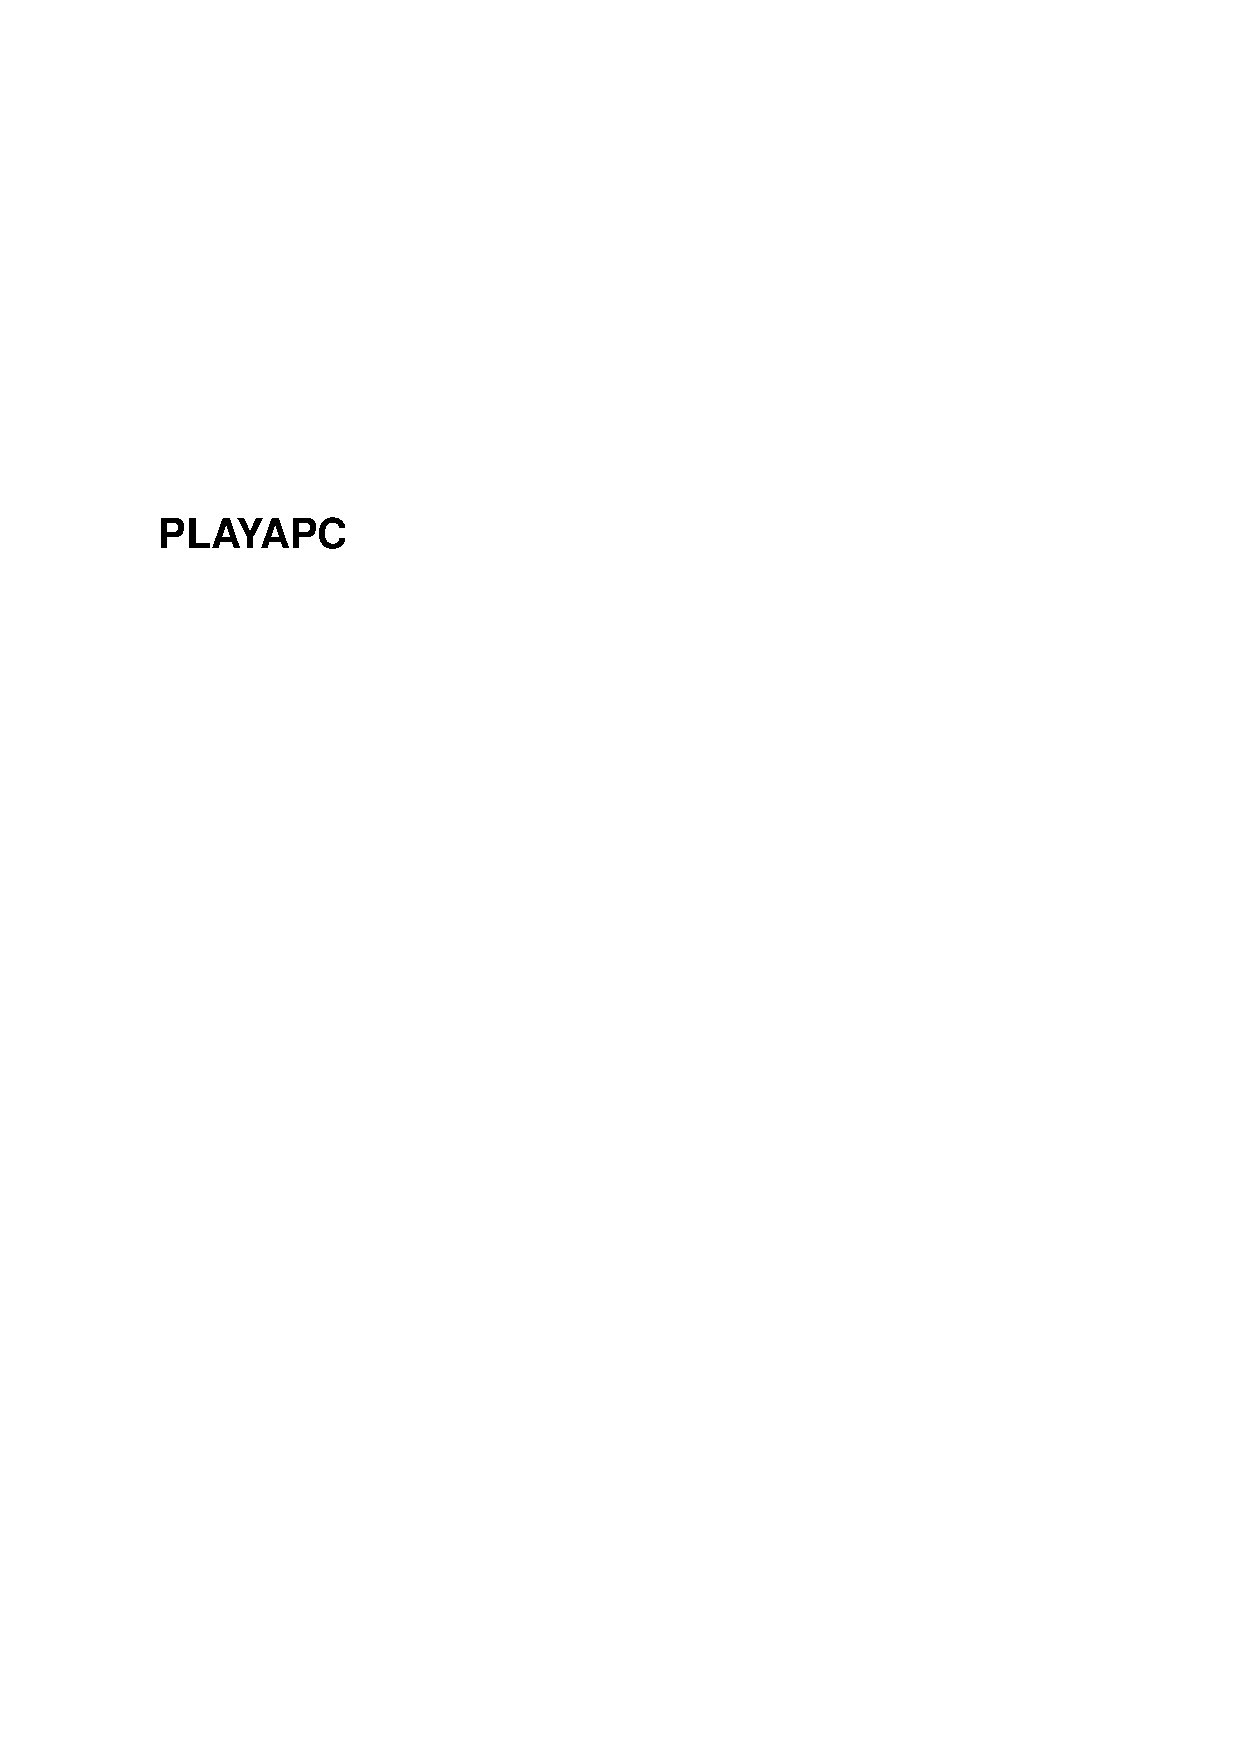
\includepdf[pages={1-}]{apendice/playcb.pdf}
A apostila de exercícios foi organizada como uma sugestão de práticas de laboratórios para os professores que queiram utilizar a biblioteca gráfica \playAPC{}. Os enunciados estão listados na Seção \ref{sec:apresentacao} e a resolução dos mesmos exercícios na Seção \ref{sec:solucoes}, com exceção do último capítulo da apostila, que contém exercícios extras. 

A estrutura da apostila está organizada em 8 capítulos.
\begin{itemize}
	\item O capítulo 1 possui 4 exercícios de algoritmos sequenciais;
	\item O capítulo 2 possui 3 exercícios de algoritmos condicionais;
	\item O capítulo 3 possui 5 exercícios de algoritmos com repetição;
	\item O capítulo 4 possui 2 exercícios de vetores;
	\item O capítulo 5 possui 3 exercícios de matrizes;
	\item O capítulo 6 possui 3 exercícios de função;
	\item O capítulo 7 possui 4 exercícios de recursão;
	\item O capítulo 8 possui 3 exercícios extras;
\end{itemize}

O capítulo 8 possui exercícios que referenciam os demais capítulos, envolvendo todos os tópicos abordados do 1 ao 7.
